\usetikzlibrary{calc}
\begin{frame}{concept: labels and control flow graph}
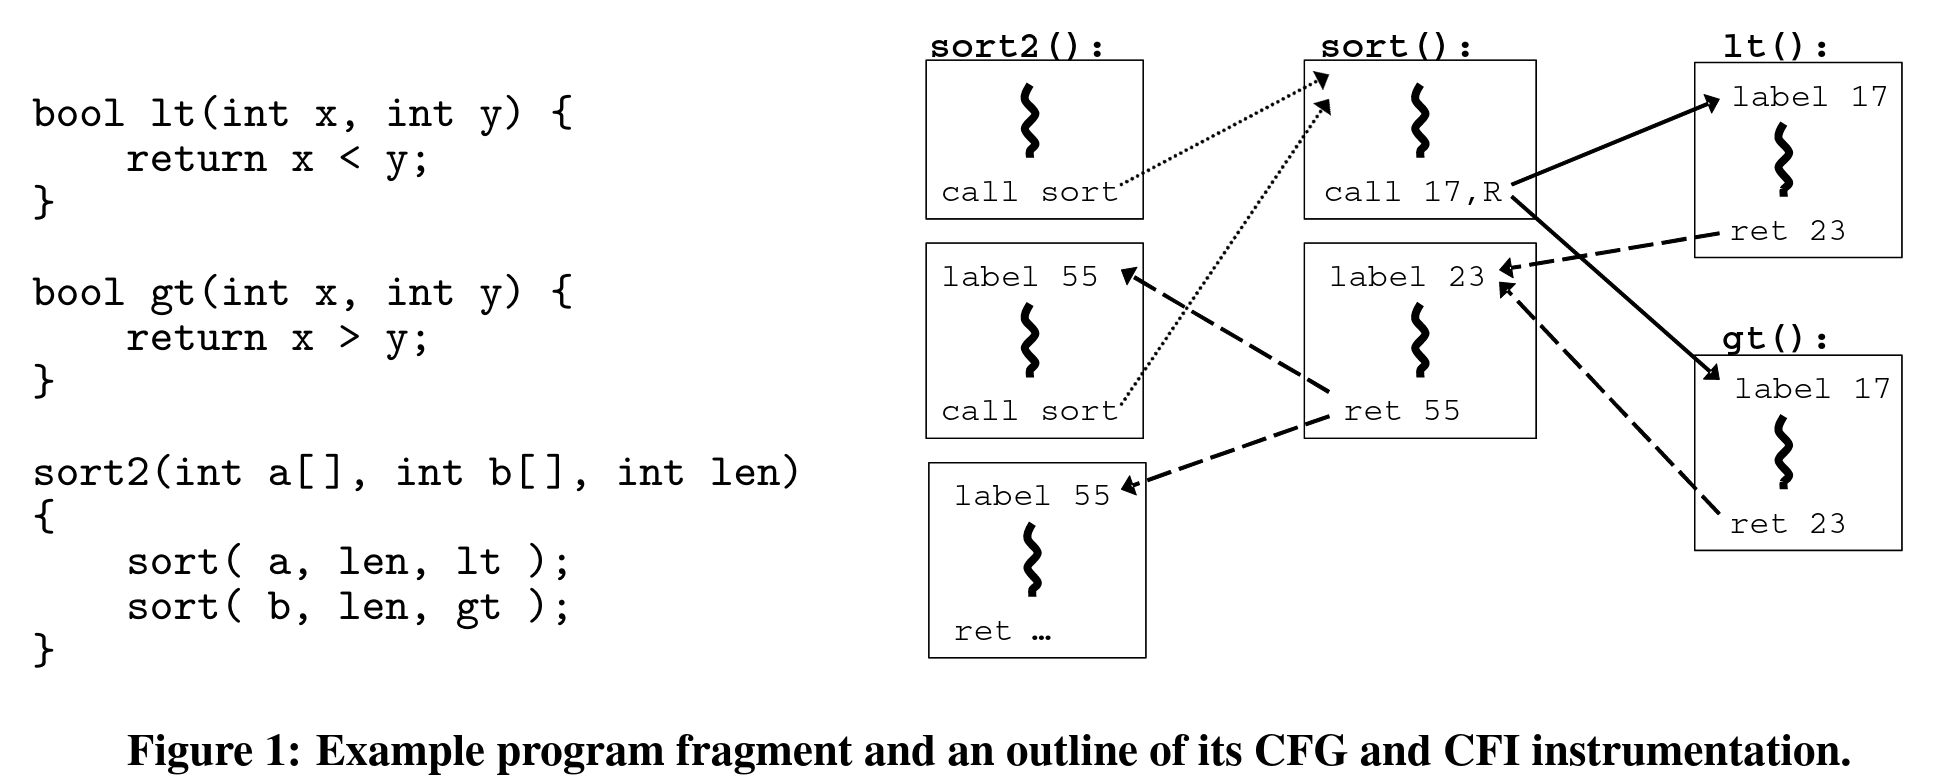
\includegraphics[width=0.7\textwidth]{../cfi/abadi-fig1}
\begin{itemize}
\item control flow graph
    \begin{itemize}
    \item nodes = blocks of code
    \item edges = \textit{potential jump/call}
    \end{itemize}
\item assigning labels: every in-edge needs to check same label at source
\end{itemize}
\imagecredit{figure from Abadi et al, ``Control-Flow Integrity: Principles, Implementations and Applications'' (CCS 2005)}
\end{frame}

